\documentclass{article}

\usepackage[numbers]{natbib}  % For citation management - numbers style matches current format
\usepackage{subcaption}  % Add this to preamble if not already present
\usepackage{fancyvrb}
\usepackage{amsmath,amssymb}
\usepackage{graphicx}
\usepackage{listings}
\usepackage[ruled,vlined]{algorithm2e}
\usepackage{xcolor}
% Add to preamble:
\usepackage{listings}
\usepackage{xcolor}

% Define colors for syntax highlighting
\definecolor{codebackground}{rgb}{0.98,0.98,0.98}
\definecolor{codegray}{rgb}{0.5,0.5,0.5}
\definecolor{codepurple}{rgb}{0.58,0,0.82}
\definecolor{codegreen}{rgb}{0.25,0.5,0.37}
\definecolor{codekeyw}{rgb}{0.23,0.49,0.73}

% Full definition of Scheme language for listings
\lstdefinelanguage{Scheme}{
    morekeywords={define, lambda, if, cond, else, let, and, or, map, 
                  begin, quote, car, cdr, cons, list, null, set!, 
                  apply, eval, display, newline},
    sensitive=true,
    morecomment=[l]{;},
    morestring=[b]",
    basicstyle=\ttfamily\footnotesize,
    keywordstyle=\color{codekeyw}\bfseries,
    commentstyle=\color{codegray},
    stringstyle=\color{codepurple},
    showstringspaces=false
}

% Set up code listing style
\lstset{
    % Reduced font size and adjusted line spread
    basicstyle=\linespread{1.1}\ttfamily\footnotesize,
    backgroundcolor=\color{codebackground},
    commentstyle=\color{codegray},
    keywordstyle=\color{codekeyw}\bfseries,
    stringstyle=\color{codepurple},
    numberstyle=\tiny\color{codegray},
    breakatwhitespace=false,
    breaklines=true,
    captionpos=b,
    keepspaces=true,
    numbers=left,
    numbersep=8pt,  % Reduced number separation
    showspaces=false,
    showstringspaces=false,
    showtabs=false,
    tabsize=2,
    frame=leftline,
    framesep=6pt,  % Reduced frame separation
    framexleftmargin=10pt,
    framextopmargin=4pt,
    framexbottommargin=4pt,
    % Adjusted margins to use more horizontal space
    xleftmargin=15pt,
    xrightmargin=2pt,  % Reduced right margin
    aboveskip=16pt,
    belowskip=16pt,
    emphstyle={\color{codekeyw}},
    morekeywords={env, args, node},
    % Better line breaking settings
    breaklines=true,
    breakatwhitespace=true,
    prebreak=\raisebox{0ex}[0ex][0ex]{\ensuremath{\hookleftarrow}},
    columns=flexible  % Better spacing for code
}

% Language-specific adjustments
\lstdefinestyle{pythonstyle}{
    language=Python,
    morekeywords={self, return, yield, raise, break, continue, pass, assert},
    commentstyle=\color{codegray},
    stringstyle=\color{codepurple},
}

\lstdefinestyle{xmlstyle}{
    language=XML,
    morekeywords={xmlns,xml,version}
}

\lstdefinestyle{schemestyle}{
    language=Scheme
}
\title{Intelligent Automation for Scientific Workflows}
%\author{Oliver Hoidn} % Replace with actual author name
\date{}

\usepackage[hidelinks]{hyperref}
\begin{document}
\maketitle


Scientific facilities like SLAC face a key challenge: as experimental capabilities grow more sophisticated, the complexity of data analysis and decision-making increases dramatically. Modern AI systems, particularly Large Language Models (LLMs), offer promising capabilities for automation and assistance but face fundamental limitations when applied to demanding scientific workflows.

This section of the research program proposes a novel approach inspired by classical ideas from programming language implementation, particularly the metacircular evaluator concept from Lisp and the staged compilation techniques from modern compilers. I will argue that the LLM should be treated as a basic component of a larger system that can, if built in a certain way, be much more capable than the underlying LLM. 

If successful, the system would provide a foundation for better AI-assisted scientific workflows, enabling more aggressive automation efforts across SLAC's experimental facilities. The resulting research innovations might also give compounding returns by encouraging collaboration with the broader AI / ML research.

%\subsection{Current State and Limitations}
%Current approaches to ML-based agents in scientific settings typically focus on narrow, specialized tasks or attempt to use general-purpose LLMs as conversational assistants. While valuable, the latter tools hit fundamental barriers when faced with:
%\begin{itemize}
%    \item Reasoning requiring coherence over a series of many steps
%    \item Large inputs that exceed model context limits
%    \item Workflows needing reproducible, verifiable results
%\end{itemize}
%
%Traditional agent frameworks and tool-use architectures provide partial solutions but lack structured approaches to task decomposition and context management. They often rely on ad-hoc combinations of prompting techniques and external tools, leading to brittle solutions that scale poorly.

\subsection{Example: LLM-Assisted Analysis at XPP}
In the last year, I developed an automated analysis pipeline for LCLS's X-ray Pump-Probe (XPP) instrument, working with my PI (Apurva Mehta) and the LCLS analytics group. The pipeline (figure \ref{pipeline}) finds CDW signals through a contrast-enhancing transformation of the raw data and uses statistical criteria to maximize signal to noise with respect to the analysis parameters.


\begin{figure}[htbp]
    \centering
    % First row
    \begin{subfigure}{0.45\textwidth}
        \centering
        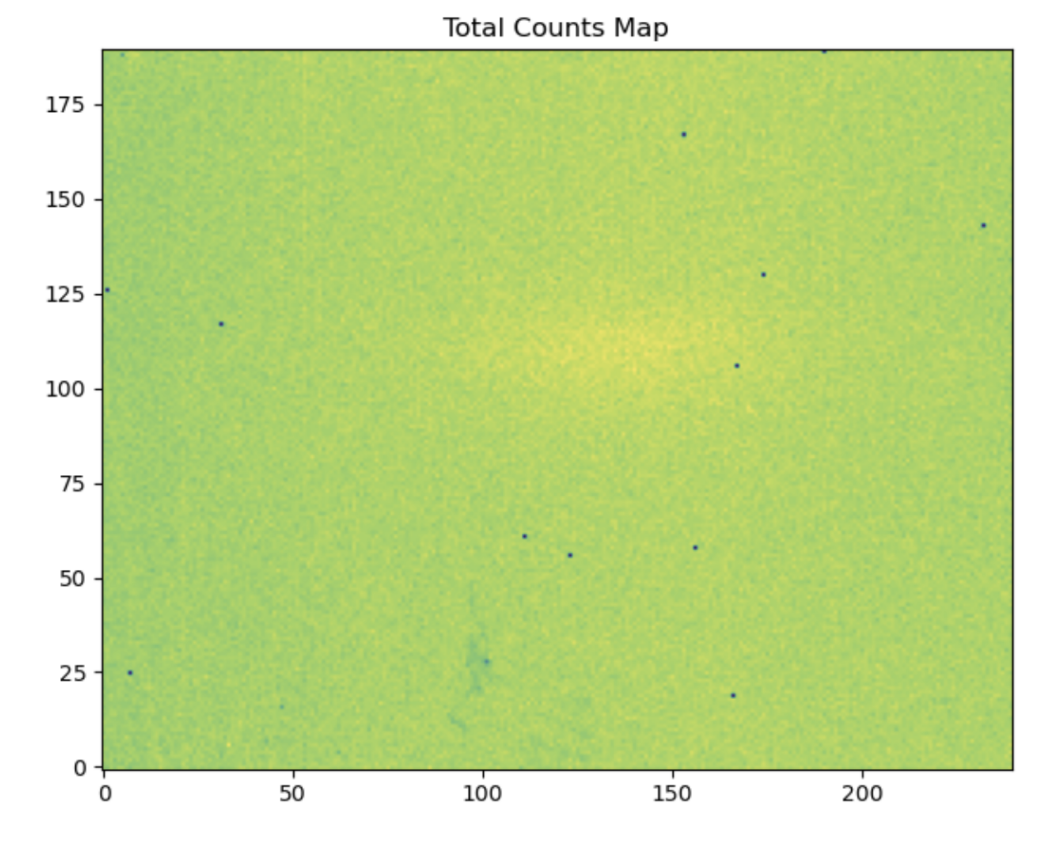
\includegraphics[width=\textwidth]{raw.png}
        \caption{}
        \label{fig:raw}
    \end{subfigure}
    \hfill  % Add horizontal space between subfigures
    \begin{subfigure}{0.45\textwidth}
        \centering
        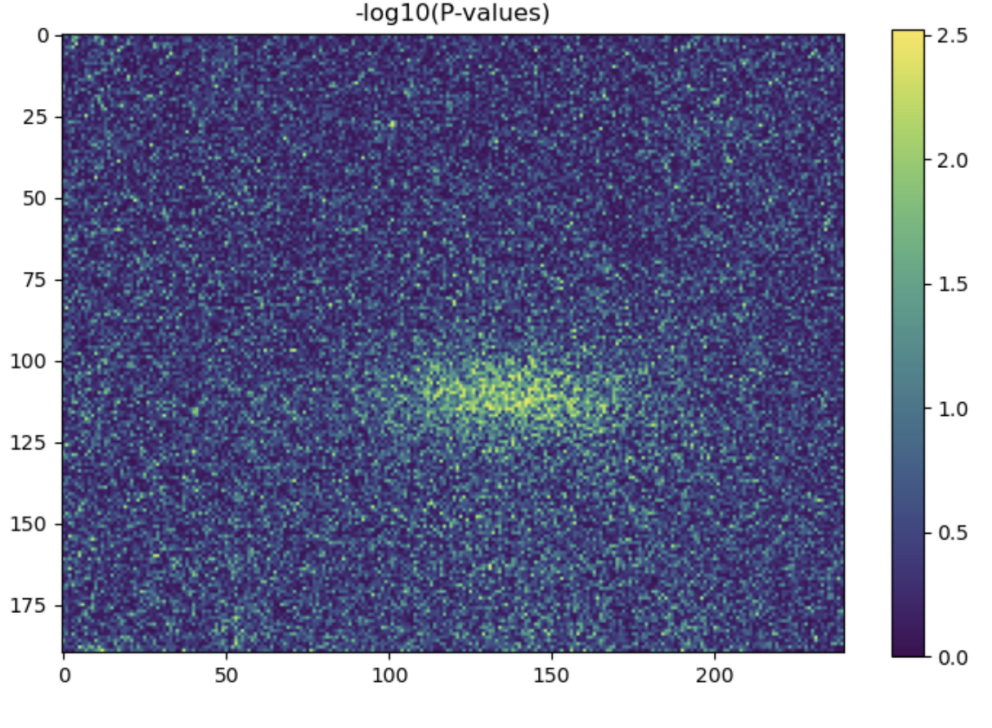
\includegraphics[width=\textwidth]{highcontrast.png}
        \caption{}
        \label{fig:highcontrast}
    \end{subfigure}
    
    \vspace{0.5cm}  % Vertical spacing between rows
    
    % Second row
    \begin{subfigure}{0.45\textwidth}
        \centering
        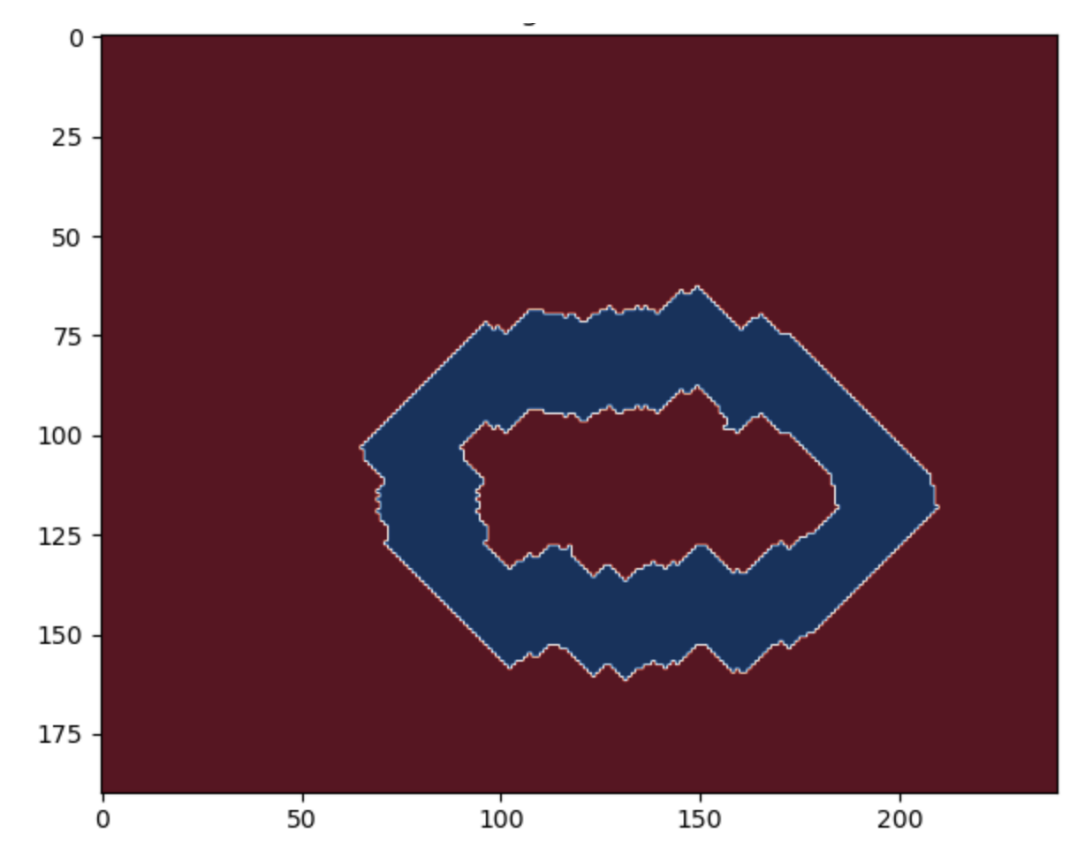
\includegraphics[width=\textwidth]{mask.png}
        \caption{}
        \label{fig:mask}
    \end{subfigure}
    \hfill  % Add horizontal space between subfigures
    \begin{subfigure}{0.45\textwidth}
        \centering
        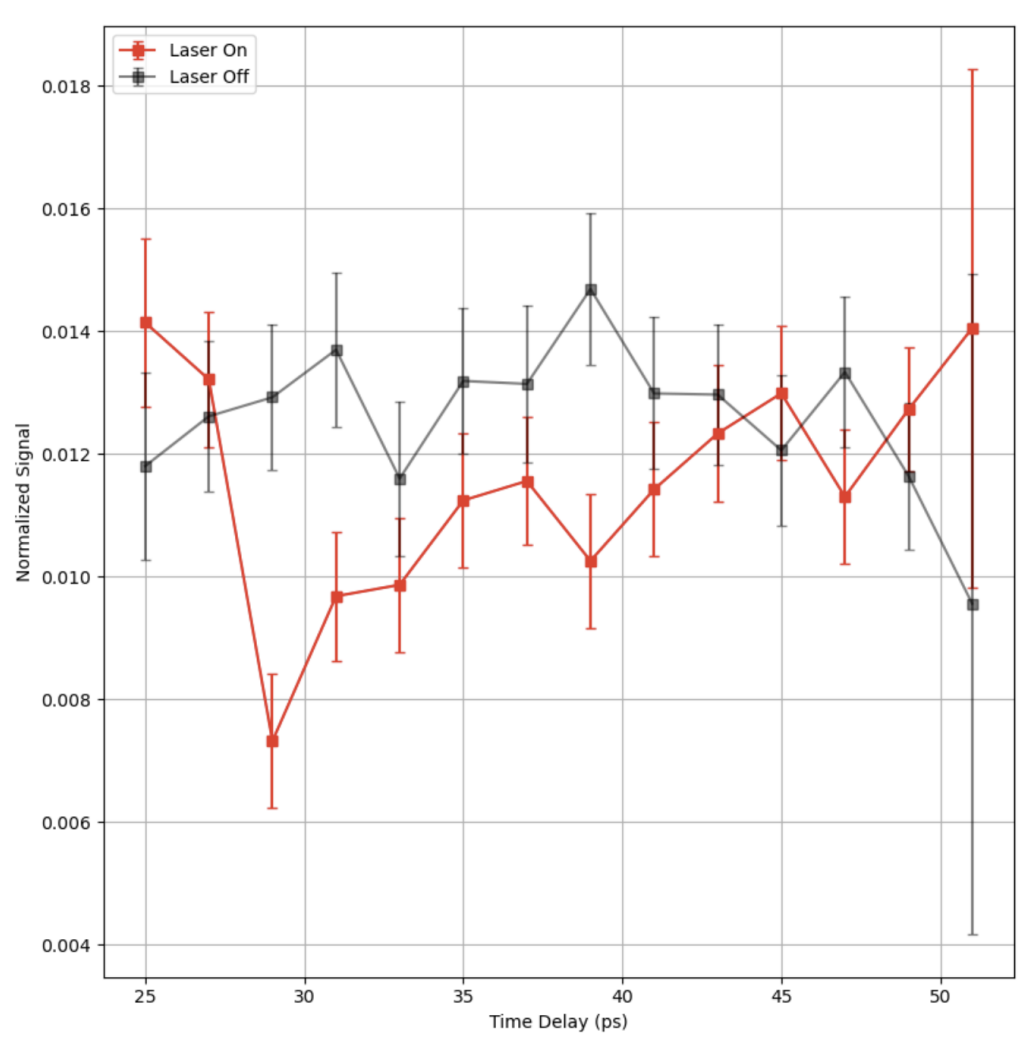
\includegraphics[width=\textwidth]{delaycurves.png}
        \caption{}
        \label{fig:delaycurves}
    \end{subfigure}
    
    \caption{In low signal-to-background settings background estimation is nontrivial, as is identifying and integrating diffraction peaks (a). Our automated workflow enhances contrast using spectral distribution statistics (b), identifies a bounding mask for the signal ((c), interior red region), estimates background levels, and finally generates a pump-probe delay curve (d). Automatic optimization of the workflow parameters yields better signal to noise than the traditional (manual) analysis.}\label{pipeline}
    \label{fig:analysis}
\end{figure}
This automation approach reduces the user's responsibility to a single numerical input: a region of interest (ROI) on the detector. While this usage is simple, interpreting diagnostic outputs when things go wrong still requires domain expertise. To address this limitation, I experimented with a language model agent to guide users through the diagnostics. In one test, I initialized the analysis with incorrect ROI coordinates. The agent reviewed logged diagnostics and successfully identified the issue:

    \vspace{0.3cm}
    \begin{Verbatim}[fontsize=\small,frame=single]
User: The pump-probe curve for the current run looks weird. What might
be wrong?

Agent: Based on the p-value uniformity check results, the designated 
background ROI [80, 95, 5, 45] appears to contain signal when it should 
not.                                                                    
This is evidenced by:

 1 Mean p-value of 0.394 (should be 0.5)
 2 Highly significant KS test (p=6.496e-17)
 3 Large z-score deviation (9.0)

This contaminated background ROI would affect the null distribution     
calculation, which in turn would distort the pump-probe curve. The      
solution would be to select a different background ROI location that    
shows proper uniformity in its p-values.
    \end{Verbatim}


While effective for modest diagnostic tasks, the system revealed fundamental limitations in more difficult situations. Attempting to use it for analyzing large collections of log files or guiding multi-step decision processes exposed a well-known underlying limitation of LLMs: difficulty maintaining analytical context across multiple interaction turns, especially when handling large datasets. This limitation is exacerbated by how LLMs perform reasoning itself - since techniques like reflection and chain of thought demonstrate that LLM `thought' operates through token generation, each step of analysis consumes valuable context window capacity.


\section{Technical Innovation: A Language-Model Architecture for Scientific Computing}
Such limitations point to a deeper challenge: we lack supporting tools for constructing agent systems in scientific environments because the underlying kernel of a natural language agent -- the LLM itself -- is on its own insufficient. Conventional automation at light sources depends on robust software design --  similarly, we will need principled architectures for composing natural language agents into scientific workflows with sufficient scale, capability and robustness.

%Scientific computing workflows demand analytical capabilities coupled with standards for reproducibility and verification. Current language model architectures, while powerful and versatile, face fundamental limitations when applied to scientific tasks. Fixed context windows put a practical cap on the amount of analysis possible within a single LLM session, as does the gradual degradation in model performance as the context window fills with output tokens.

The last two years have seen rapid growth in LLM-based agent frameworks like AutoGPT and BabyAGI. While useful, these systems rely on ad-hoc combinations of prompts and tools, making them brittle, inconsistent and hard to extend. Rather than systematically addressing the key limitations of LLMs, these agentic approaches reproduce or even compound them. A case in point is reliance on techniques such as retrieval-augmented generation (RAG) that aim to compensate for limited context window capacities but introduce serious tradeoffs in recall and accuracy.

I suggest an alternative that takes inspiration from two fundamental concepts in programming language implementation: the metacircular evaluator pattern first developed for Lisp, and staged compilation techniques used in modern compilers.

The main insight is treating natural language interaction with an LLM as a form of code execution. Suppose that we first ask the LLM to translate natural language instructions into programs written in a DSL (domain specific language). The structure of such a DSL program will represent the decomposition of a complex prompt into multiple tasks. The interpretation of the same program involves distribution of each component task to an LLM instance and the linking together of instances through a calling convention and shared memory system.

More concretely:

\begin{algorithm}[H]
\SetAlgoLined
\SetKwInOut{Input}{Input}
\SetKwInOut{Output}{Output}
Natural Language Query\;
$\downarrow$ [LLM Translation]\;
XML Task Structure (equivalent to S-expression)\;
$\downarrow$ [Parser]\;
Abstract Syntax Tree\;
$\downarrow$ [tree traversal]\;
LLM execution\;
\caption{System Overview}
\end{algorithm}

In this schema, natural language queries are first translated into composite expressions made up of smaller units (atomic tasks) with the purpose to make the execution tractable while preserving semantics of the original query. A satisfying feature of the setup is that it will be self-hosting in the sense that the LLM evaluates DSL procedures generated by the LLM.

An equivalent perspective is that the framework will dynamically compile the user's prompt into a directed acyclic graph (DAG). Each node of the DAG is dispatched to a separate LLM session, and data travels down and up the nodes of the graph in the form of environment frames and return values, respectively. 

The architecture consists of three main components:

\newpage
\subsection{Execution Model}
Two mutually recursive procedures, eval and apply, work with each other to evaluate DSL expressions:


\begin{lstlisting}[language=Scheme, caption = Scheme sketch of the evaluation procedure]
; Evaluates a task in the given environment; returns direct result or decomposed tasks
(define (eval-task task env)
  (cond 
    ; For atomic tasks, try direct application; if it fails, decompose
    ((atomic? task)
     ; amb tries the first option; if it fails, backtracks to the second
     (amb (apply-proc task '() env)                 ; Direct application
          (eval-task (decompose task) env)))        ; Or decomposition
    
    ; For compound tasks: evaluate arguments, apply procedure
    (else 
     (let ((proc (task-proc task))
           (args (map (lambda (arg) (eval-task arg env))
                     (task-args task))))
       (apply-proc proc args env)))))

; Applies a procedure to evaluated arguments in given environment
(define (apply-proc proc args env)
  (cond
    ; For primitives, try direct execution; if it fails, decompose and retry
    ((primitive? proc)
     ; amb tries the first option; if it fails, backtracks to the second
     (amb (execute-llm proc args env)               ; Direct execution
          (eval-task (decompose proc args) env)))   ; Or decomposition
    
    ; For compound procedures: create new environment, evaluate body
    (else
     (let ((new-env (extend-environment proc args env)))
       (eval-task (procedure-body proc) new-env)))))
\end{lstlisting}

When task execution ends with an error (e.g. context window overrun, output validation failure), the executor can retry by generating and evaluating an alternate procedure -- for example, a decomposition of the task into multiple subtasks.

The creation of the execution data context 'env' is mediated by the memory subsystem.

\subsection{Associative memory system}
The memory system explicitly separates storage and working contexts through a hierarchical design:
\begin{itemize}
    \item Long-term memory for data and procedures
    \item Working memory for active computations
    \item Context frames that capture execution environments (including working memory)
\end{itemize}

Working memory is instantiated from long-term storage using an associative retrieval mechanism that is itself an (atomic) LLM procedure whose purpose is to match an atomic task to a contextually relevant subset of the data in long-term memory.

\subsection{Task Expression Framework}
The expression system supports nested procedures and basic functional patterns:

\begin{lstlisting}[caption=Task Expression Types]
AtomicTask     -> Direct LLM execution
NestedTask     -> Compositional evaluation  
MapExpression  -> Parallel processing
ReduceExpression -> Result combination
\end{lstlisting}

These expressions, which can be extended, provide formal semantics for the DSL.

\section{Implementation Plan}
The implementation strategy builds on recent work and collaborations at SLAC. Working with LCLS beamline scientist Lingjia Liu and Frederic Poitevin from the LCLS analytics group, I developed the previously mentioned analysis approach for charge density wave dynamics in pump-probe experiments. The project aligns with broader LCLS initiatives, led by Jana Thayer and others, to develop real-time analysis capabilities for experimental beamlines.

Building on these experiences and collaborations, the implementation will proceed in two phases:

First, we will develop the core architectural components: the memory system for managing analysis contexts, the execution model for task decomposition, and initial task libraries. These libraries will include specialized agents for software architecture, code generation, analysis refinement, and experimental log interpretation. We'll work with the LCLS analytics group to ensure the framework complements their efforts, and with beamline scientists to get feedback from the end-user point of view.

Second, we will focus on development across scientific workflows based on reusable task patterns that combine automated processing with human-in-the-loop guidance. The framework will support diverse needs, from real-time experiment optimization to offline analysis and documentation. The goals will include accelerated analysis turnaround and reduced downtime during beamtimes.

\section{PL concepts and concrete examples}
\subsection{Compilation}

Staged compilation traditionally refers to breaking down compilation into distinct phases, where each stage transforms the program into a new representation closer to the target execution form:

\begin{verbatim}
Source code → Parse tree → AST → Intermediate code → Machine code
\end{verbatim}

%Our system adapts this concept for LLM task execution. Instead of fixed transformations between predefined languages, we use the LLM itself to generate intermediate representations. 




Our system uses the LLM to parse natural language into structured expressions:

\emph{TODO this is incomplete. There should be a cycle connecting 'Task executable' back to 
'AST', to represent dynamic / incremental reparsing. See also: the other TODOSs, <dynamic reparsing>}
\begin{verbatim}
Source code (English) → Parse tree (XML) → AST (Python) → Task data + executable (XML) 
\end{verbatim}

In Python the first three steps (\verb|Source code (English) → Parse tree (XML) → AST (Python)|) are orchestrated by the class Compiler. The remaining portion is generated by the interaction between Compile and the evaluation loop (see Evaluator, next section):

\begin{lstlisting}[language=Python]
from dataclasses import dataclass
from typing import List, Any

@dataclass
class ASTNode:
    operator: Any
    args: List['ASTNode']

@dataclass
class Operator:
    """Represents an operation to be performed"""
    type: str  # "atomic" or "compound" 
    task: str  # The actual task description
    params: Optional[Dict] = None  # Additional parameters if needed

from dataclasses import dataclass
from typing import List, Any, Optional, Dict
from enum import Enum
from xml.etree.ElementTree import Element

from .error_types import ExecutionError, ErrorType, ResourceType
from .environment import Environment
from .task_system import TaskSystem, TaskType, XMLTaskParser, TaskStructure

@dataclass
class ASTNode:
    """Represents a node in the Abstract Syntax Tree"""
    operator: Any
    args: List['ASTNode']

@dataclass
class Operator:
    """Represents an operation to be performed"""
    type: str  # Maps to TaskType values
    task: str  # Task description
    params: Optional[Dict[str, Any]] = None

from dataclasses import dataclass
from typing import Protocol, Dict, Optional
from enum import Enum
from xml.etree.ElementTree import Element

from .error_types import ResourceType, ExecutionError

class TaskSystem(Protocol):
    """Interface for task management and prompt generation"""
    
    def get_decomposition_prompt(self, task: str, resource: ResourceType) -> str:
        """Generate prompt for decomposing a task that exceeded resources
        
        Args:
            task: The task description that failed
            resource: Which resource was exhausted
            
        Returns:
            Prompt for LLM to generate decomposed task structure
        """
        ...
        
    def get_alternative_prompt(self, task: str, failure_reason: str) -> str:
        """Generate prompt for alternative approach after task failure
        
        Args:
            task: The task description that failed
            failure_reason: Why the task failed
            
        Returns:
            Prompt for LLM to generate alternative approach
        """
        ...

class TaskType(Enum):
    """Types of tasks in decomposition"""
    ATOMIC = "atomic"         # Direct LLM execution
    MAP = "map"              # Parallel subtasks
    REDUCE = "reduce"        # Combine results
    SEQUENCE = "sequence"    # Sequential steps

@dataclass
class TaskStructure:
    """Parsed representation of a task from XML"""
    type: TaskType
    description: str
    subtasks: list['TaskStructure'] = None
    parameters: Optional[Dict[str, str]] = None



\end{lstlisting}

Example task structure in XML:
\begin{lstlisting}[language=XML]
<task>
  <description>analyze peak patterns across detectors</description>
  <inputs>
    <input name="detector1_data">
      <task>
        <description>load and preprocess detector 1 data</description>
        <expected_output>
          Preprocessed detector 1 data in standard format:
          - Intensity values
          - Peak positions
          - Background levels
        </expected_output>
      </task>
    </input>
    <input name="detector2_data">
      <task>
        <description>load and preprocess detector 2 data</description>
        <expected_output>
          Preprocessed detector 2 data in standard format:
          - Intensity values
          - Peak positions
          - Background levels
        </expected_output>
      </task>
    </input>
  </inputs>
  <expected_output>
    Comparative peak analysis:
    - Peak correlations between detectors
    - Intensity pattern matching
    - Anomaly detection
  </expected_output>
</task>
    <!--
# TODO the above xml is just an example, but we need to clearly define a mapping between the 
# structure of xml generated by the llm (when it does <reparsing>) and AST subtrees. (We could 
# potentially simplify this by constraining the llm <reparsing> process so that it can only generate 
# one ASTNode at a time. In the case of composite nodes, this would mean generating xml for an outer 
# task (e.g. a reduction function) and inner task(s) (e.g. the individual tasks whose outputs the 
# reduction is operating on)
    -->
\end{lstlisting}

In summary:
\begin{enumerate}
    \item The XML stage lets the LLM express task composition and input / output conventions in a structured way
    \item XML provides the interface between LLM and the evaluator
    \item Every AST node follows a uniform structure representing operations and their arguments
    \item Composite task behavior emerges from AST semantics and atomic task behavior
    \item Atomic task behavior emerge from natural-language operator definitions, which are \emph{not} exposed at this level
    \item Environments handle local variable bindings and global working memory for LLM operations (see next section)
    \item New atomic task patterns can be added without changing the evaluator or execution system
\end{enumerate}



\subsection{Environment}

An environment represents the complete context needed to evaluate expressions. In traditional programming languages, this mostly means lexical scope---the set of variables accessible from inside a given stack frame. %Our system extends this concept to include working memory for LLM tasks.


Our environments support traditional variable scoping while also managing the short-term memory component of the LLM execution context. The basic aspects are:

\begin{lstlisting}[language=Python]
class Environment:
    def __init__(self):
        """Environment holds bindings and LLM working context"""
        self.bindings = {}    # Current variable bindings
        self.context = {}     # LLM working memory
    
    def extend(self, names, values):
        """Create new environment with additional bindings"""
        new_env = Environment()
        new_env.bindings = dict(zip(names, values))
        # The full implementation will update the context using associative
        # matching via the long term - short term memory system instead of 
        # just cloning it
        new_env.context = self.context.copy()  
        return new_env
    
    def lookup(self, name):
        """Look up value in current bindings"""
        return self.bindings.get(name)
\end{lstlisting}

This is sufficient for us to:
\begin{enumerate}
    \item Track context through nested evaluations
    \item Pass relevant state between task executions
    \item Allow the evaluator to pass around execution contexts and create new ones using the associative memory procedure
\end{enumerate}

\subsection{Metacircular Evaluator}

A metacircular evaluator is an interpreter implemented using similar fundamental operations to the ones it aims to interpret. In our context, we implement a domain-specific language (DSL) evaluator using LLM operations as one basic component of the evaluation machinery, and this evaluator in turn coordinates and executes higher-level LLM tasks.

The architecture has two key aspects. First, the environment must be a first-class data structure that can be explicitly introspected by both the evaluator and the LLM. The environment captures not just variable bindings (as in a conventional programming language implementation) but the complete context needed for task interpretation and decomposition. (In contrast, in a traditional language implementation, the execution environment is entangled with the parsing and code generation process in a rather opaque way.)

The second aspect is the self-hosting property mentioned above. The LLM provides the evaluator with primitive capabilities for generating structured output from natural language (as XML task descriptions), and for executing atomic tasks. The evaluator combines these primitive operations to implement higher-level functionality: managing execution environments, parsing and dispatching structured task descriptions, and collecting execution outputs. 

Here's the core evaluator pseudo-implemented in Python:

\begin{lstlisting}[language=Python]
from dataclasses import dataclass
from typing import List, Any, Optional
from enum import Enum

# Shared type definitions
class OperatorType(Enum):
    ATOMIC = "atomic"    # Direct LLM execution
    MAP = "map"         # Process multiple inputs
    REDUCE = "reduce"   # Combine results
    SEQUENCE = "sequence" # Execute in order

# TODO only ATOMIC operators should have (or populate) the task attribute,
# because the other operator types aren't directly llm-executable. 
# Note an asymmetry between llm parsing and llm execution: when parsing, 
# the llm is locally aware of the AST structure, but when executing the 
# llm only sees one atomic node at a time. <reparsing>
@dataclass
class Operator:
    type: OperatorType
    task: str           # Task description/prompt
    params: Dict = None # Optional parameters

%<errors>
%type ExecutionError = 
%  | { type: 'resourceExhaustion'; resource: 'turns' | 'context' | 'output' }
%  | { type: 'taskFailure'; reason: string }
%  | { type: 'incompleteTask' };
%</errors>

% see evaluator.py
\end{lstlisting}

Note that the dynamic reparsing is spread out as an interaction between Evaluator and Compiler, but it is conceptually equivalent to this simple expression from the Scheme version: 

\begin{lstlisting}[language=Scheme, caption = nondeterministic evaluation using the amb (ambiguous) operator]
...
    ; For atomic tasks, try direct application; if it fails, decompose
    ((atomic? task)
     ; amb tries the first option; if it fails, backtracks to the second
     (amb (apply-proc task '() env)                 ; Direct application
          (eval-task (decompose task) env)))        ; Or decomposition
...
\end{lstlisting}


\subsection{End-to-End Example}

Let's examine how the system handles a user request that benefits from natural language understanding:

`Review our XRD analysis and check if we chose a good background region.'

The LLM first translates this into nested tasks:

\begin{lstlisting}[language=XML]
<task>
  <description>analyze background region quality</description>
  <inputs>
    <input name="region_stats">
      <task>
        <description>extract statistics from experiment logs</description>
        <parameters>
          Extract and analyze:
          - Background region coordinates
          - Statistical test p-values 
          - Distribution uniformity metrics
        </parameters>
        <expected_output>
          Structured statistics including:
          - ROI coordinates
          - P-value series
          - Distribution metrics
        </expected_output>
      </task>
    </input>
  </inputs>
  <expected_output>
    Quality assessment including:
    - Statistical validity evaluation
    - Potential signal contamination check
    - Recommendations for improvement if needed
  </expected_output>
</task>
\end{lstlisting}

The compiler builds an AST:

\begin{lstlisting}[language=Python]
node = ASTNode(
    operator=Operator(
        type="atomic",
        task="analyze_region_quality"
    ),
    args=[
        ASTNode(
            operator=Operator(
                type="atomic",
                task="extract_stats",
                params={"instruction": "Find background..."}
            ),
            args=[]
        )
    ]
)
\end{lstlisting}

The evaluator processes this with environment handling:

\begin{lstlisting}[language=Python]
# Initialize environment with both logs and documentation
env = Environment(context={
    "log_contents": """
    2024-04-06 10:15:32 INFO: Starting analysis of run 123
    2024-04-06 10:15:33 DEBUG: Background ROI set to [80,95,5,45]  
    2024-04-06 10:15:34 DEBUG: Method: local linear
    2024-04-06 10:15:35 WARNING: High fit residuals
    2024-04-06 10:15:36 DEBUG: P-values: [0.394, 0.412, 0.378]
    ...""",
    
    "analysis_docs": """
    Background Region Quality Assessment Guide:
    - P-values should follow uniform distribution (mean approximately 0.5)
    - KS test should show p > 0.05
    - Region should be at least 20 pixels from any peak
    - Common failure modes:
      * Signal contamination causes p-value clustering
      * Edge effects near beam stop distort background
    ..."""
})

# Evaluate full expression
result, final_env = evaluator.eval(node, env)

# The evaluation proceeds:
# 1. Inner extract_stats task receives filtered environment:
#    env.context = {
#        "log_contents": "..." # Only the log data needed for extraction
#    }
#    -> Returns structured data like:
#       {"roi": [80,95,5,45], 
#        "pvalues": [0.394, 0.412, 0.378]}

# 2. Outer analyze_region_quality task receives full context:
#    env.context = {
#        "analysis_docs": "...", # Documentation for analysis guidance
#        "extraction_results": {"roi": [80,95,5,45], ...}
#    }
#    -> Uses docs to guide analysis:
#       "Background region shows signs of signal contamination.
#        P-value clustering (mean=0.394) matches known failure mode
#        described in analysis guide."
\end{lstlisting}

In this example, each task gets minimal context needed for its operation and the outer tasks can access both the log-parsing results (as direct input) and reference documentation (as context / short-term memory).

\end{document}

